\chapter{Extensions of Tubularity Flow Field} 

\label{AppendixLDE} % For referencing this appendix elsewhere, use \ref{AppendixA}

\lhead{Appendix B. \emph{TuFF applications}} % This is for the header on each page - perhaps a shortened title

Tubularity Flow Field is  designed  specifically for neuron segmentation, both in 2D and 3D. However, since the basic formulation of TuFF (see (TuFF formula)) can be extended for segmenting any vascular structure,  and is not particularly  restricted to neurons only. Segmenting vascular structures is a salient problem in the biomedical imaging literature. Sample applications include, but are not limited to, segmenting arteries and veins from magnetic resonance angiography (MRA) images of different organs such as brain, liver, retina etc. 

For neuron segmentation, the major hurdle was to accommodate the complicated filamentous architectures, along with the ability to handle structure gaps due to heterogeneous florescence. However, it should be noted that our neuron segmentation example is restricted to single cell analysis only, and the attraction force term in TuFF may produce undesirable effects when multiple  filamentous structures are present. Therefore, to generalize TuFF for applications other than neuron tracing, we need replace the attraction force term with other means to handle filament bifurcations and intensity  attenuation.

Also, in applications where the filament edges are prominent (i.e. if the gradient magnitude at the boundaries are significant), segmentation accuracy can be further improved by incorporating a edge based energy in TuFF energy equation. This results in better adherence to object edges and reduces the leakage phenomenon. The modifications suggested in this appendix are focused at the two above mentioned points:
\begin{itemize}
 \item A robust method to enhance heterogeneously  illuminated filaments, and other structure patterns such as sharp bends and bifurcations. 
 \item A solution to incorporate edge information in the TuFF energy functional to avoid leakage in low contrast images.
\end{itemize}


\section{Vessel Contrast Enhancement With Local Directional Evidence}
\begin{figure}[t]
\centering
%\renewcommand{\tabcolsep}{0.05cm}
\begin{tabular}{c}
	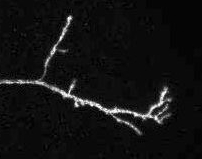
\includegraphics[width=.3\textwidth]{./images/LDE/n13} \\
	\scriptsize (a) \\
\begin{tabular}{cc}
		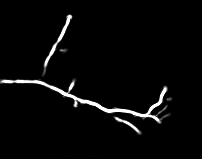
\includegraphics[width=.3\linewidth]{./images/LDE/n13_enh_frangi} &
		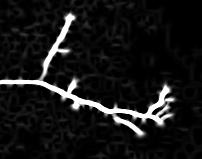
\includegraphics[width=.3\linewidth]{./images/LDE/n13_enh_our} \\
		\scriptsize (b1) & 		\scriptsize (b2) \\
		\includegraphics[width=.3\linewidth]{./images/LDE/n13_frangi_cyan_rect} &
		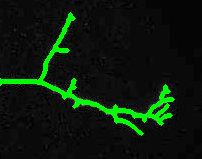
\includegraphics[width=.3\linewidth]{./images/LDE/n13_ours} \\
		\scriptsize (c1) & 		\scriptsize (c2) 
\end{tabular}
\end{tabular}
\caption{ (a) A confocal microscopy image of a dendrite is shown in the first row. (b1) Shows the results of vessel enhancement due to Frangi's filter\cite{frangi_vesselness} and (b2) shows the enhancement via LDE. (c1) The segmented centerline using \cite{frangi_vesselness} is displayed in cyan and (c2) the tracing via LDE is shown in green. Segmentation errors using \cite{frangi_vesselness} are highlighted by the yellow rectangles. }
\label{fig:demo_comp}
\end{figure}
Previously, we have discussed the vessel enhancement method due to Frangi \cite{frangi_vesselness}, which performs eigen analysis of the multiscale hessian matrix of the image to identify and enhance filamentous objects.  However, this popular vessel enhancing algorithm suffers from some deficiencies. First, intensity variation across the vessels compromises the enhancement result. This is primarily because the algorithm is inherently local and does not utilize neighboring vessel evidence. Furthermore, the method of \cite{frangi_vesselness} assumes that the vessel filaments can be approximated as an ellipsoid, an assumption which is violated  at bifurcation and vessel bends (see Fig.~\ref{fig:demo_comp}). As a result, the output of this vesselness filter sometimes requires an additional postprocessing such as vessel diffusion \cite{manniesing2006vessel}, tensor voting \cite{roysam_tensorvoting} etc.

\subsection{Vessel detection with oriented filters}
Vessel detection problem can be posed as finding the maximum response when the image is convolved with a suitable template (see Fig.~\ref{fig:templates}(b-c)) at multiple orientations.  Freeman and Adelson \cite{freeman1991steerable} introduced a class of filters, namely steerable filters, which can be rotated by taking a linear combination of a few  basis filters. For ridge detection, steerable filters based on second order derivatives of the gaussian function are popular due to computational simplicity. Jacob and Unser\cite{jacob2004steerable} showed that efficient ridge templates can be computed using directional gaussian second derivatives. The hessian  $H_\sigma(p)$ of a 2-d image $f(p)$, convolved with a gaussian kernel $g(p;\sigma)=\dfrac{1}{\sqrt{2\pi}\sigma}e^{-\frac{x^2+y^2}{2\sigma^2}}$ at a position $p=(x,y)$ is given by 
\bea
H_\sigma(p)= \left( \begin{array}{cc} 
g_{xx}(p) & g_{xy}(p) \\
g_{xy}(p) & g_{yy}(p)
\end{array} \right)* f(p)       
\eea
\begin{figure}[t]
\centering
\renewcommand{\tabcolsep}{0.05cm}
	\begin{tabular}{@{}ccc @{}}
		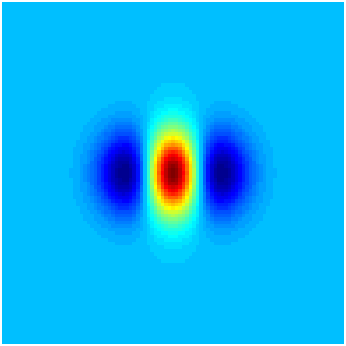
\includegraphics[width=.25\linewidth]{./images/LDE/r_d} &
		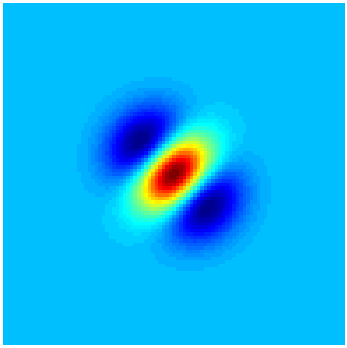
\includegraphics[width=.25\linewidth]{./images/LDE/r_d_45} &
		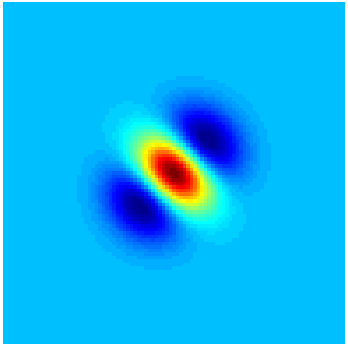
\includegraphics[width=.255\linewidth]{./images/LDE/r_d_135} \\
		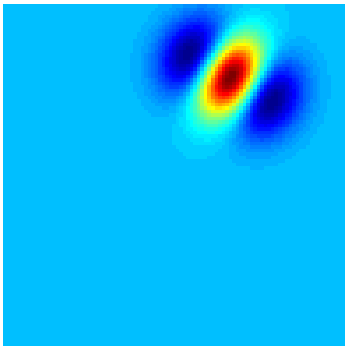
\includegraphics[width=.255\linewidth]{./images/LDE/r_f} &
		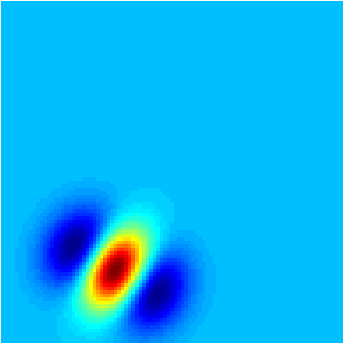
\includegraphics[width=.255\linewidth]{./images/LDE/r_b} &
		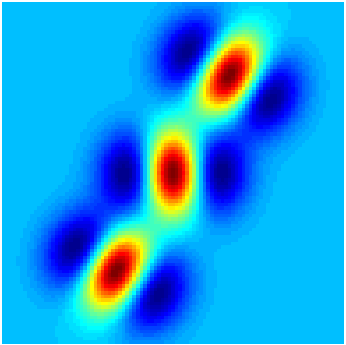
\includegraphics[width=.255\linewidth]{./images/LDE/all} \\
	\end{tabular}
\caption{The top row shows oriented vessel detector kernels $r_d$ for $\theta=0,\frac{\pi}{4},-\frac{\pi}{4}$	from left to right. The bottom row shows from left to right: forward evidence kernel $r_f$, backward evidence kernel $r_b$ and the superimposed LDE kernels for $\theta=0$ and $\psi_1=\psi_2=\frac{\pi}{6}$. We choose the offset to an exaggerated value $d=4\sigma$ for improved visual clarity.}
\label{fig:templates}
\end{figure}
The second derivative of the smoothed image in a direction $\textbf{u}_\theta=\left(\cos\theta,\sin\theta \right)^T$ is obtained as
$ \mathcal{R}_d(p,\theta;\sigma) = \textbf{u}^T_\theta H_\sigma(x,y)\textbf{u}_\theta $. Simplifying this, we obtain the directional vessel response as follows:
\bea
&\mathcal{R}_d(p,\theta;\sigma)= r_d(p,\theta;\sigma)*f(p) \\
&r_d(p;\theta,\sigma)= g_{xx}\cos^2\theta+g_{yy}\sin^2\theta+g_{xy}\sin2\theta
\label{eq:oriented_ridge}
\eea
The vesselness score at scale $\sigma$ is computed as
\bea
\mathcal{R}_d^*(p;\sigma)=\max_{\theta}\mathcal{R}_d(p,\theta;\sigma)
\label{eq:vesselness_detector}
\eea
Here $r_d(p;\sigma,\theta)$ denotes a local vessel detector template, oriented at an angle $\pi/2+\theta$. A higher value of the inner product of the shifted and rotated version of the template $r_d(p,\theta;\sigma)$ at each image pixel provides evidence for presence of a vascular object orientated at an angle $\theta$ and scale $\sigma$. A set of three detector kernels are shown in Fig.~\ref{fig:templates}, top row. Despite the  property of  steerability of the local detection template $r_d$, such detectors are prone to local intensity variation across the vascular structures. Moreover, the designed steerable kernel in (\ref{eq:oriented_ridge}) is suited for detecting homogeneous vessels and is incapable of handling complicated structures such as vessel bifurcations. 

The motivation for this work comes from the fact that the widely used vessel enhancing filters \cite{frangi_vesselness,wilkinson2001shape,sato1998three,krissian2000model} are less adept at detecting vascular regions of low intensity and bifurcation points. Our proposed method, called Local Directional Evidence (LDE), uses a set of oriented filters to determine local evidence of vessels. This set of oriented filters, in addition to the local detector filter shown in (\ref{eq:vesselness_detector}) is used to enhance low contrast vascular structures with complicated morphology. 

\subsection{Vessel enhancement with local directional evidence (LDE)}

As mentioned before, a major defect with current vessel enhancement methods is the inability to tackle local intensity variations and complex morphology. This creates further artifacts during segmentation, where multiple fragments are created which again require further connectivity analysis \cite{mukherjee_T2T_2,basu_T2T_journal}. We hypothesize that one possible way to handle this problem is to boost the local detector response (\ref{eq:oriented_ridge}) with evidence of a vessel in a given local  neighborhood.

The local directional evidence is provided by convolving the image with another set of oriented filters-- forward filters $r_f(p;\sigma,\psi_1)$ and backward filters $r_b(p;\sigma,\psi_2)$. We compute the set of local evidence filters in the following manner:
\bea
r_f(p;\sigma,\psi_1)=r_d(x+d\cos(\theta+\psi_1),y+d\sin(\theta+\psi_1)) \\
\label{eq:r_f}
r_b(p;\sigma,\psi_2)=r_d(x-d\cos(\theta+\psi_2),y-d\sin(\theta+\psi_2))
\label{eq:r_d}
\eea
Here $\theta-\alpha\le \psi_1,\psi_2 \le \theta+\alpha$ is a set of orientations used to detect evidence of vessels in a local angular region near the detection point. The offset parameter $d>0$ controls the locality of the evidence filters. While a low value of $d$ does not contribute enough, a significantly larger value may introduce false positives by predicting vessels which do not belong to the same structure. For experimental evaluation, we choose $\alpha=\frac{\pi}{3}$ since abrupt bending in vessels is rare in our applications (neurons and retinal blood vessels). The value of $d\leq\sqrt{2}\sigma$ has been observed to give good balance between localization and accuracy of the evidence filters. A set of evidence kernels is shown in the second row of Fig.~\ref{fig:templates} with $\theta=0$ and $\psi_1=\psi_2=\frac{\pi}{6}$.

The response due to the evidence kernels are given by $\mathcal{R}_f(p;\sigma,\psi_1)= r_f(p;\sigma,\psi_1)*f(p)$ and $\mathcal{R}_b(p;\sigma,\psi_2)= r_b(p;\sigma,\psi_2)*f(p)$. The overall vessel enhancement response is calculated in the following manner:
\bea
\mathcal{R}^*(p;\sigma)=\max_{\theta} \mathcal{R}_d(p)+\mathcal{R}^*_b(p)+\mathcal{R}^*_f(p)\\
\mathcal{R}^*_b (p)=\max_{\psi_1}\mathcal{R}_b(p) \; \text{and} \; \mathcal{R}^*_f (p)=\max_{\psi_2}\mathcal{R}_f(p) \nn
\label{eq:total_sum}
\eea
\begin{figure}[t]
\centering
\renewcommand{\tabcolsep}{0.05cm}
\begin{tabular}{@{}ccc@{}}
		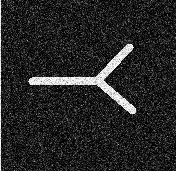
\includegraphics[width=.3\linewidth]{./images/LDE/sim2} &
		\includegraphics[width=.3\linewidth]{./images/LDE/sim2_frangi_resp} &
		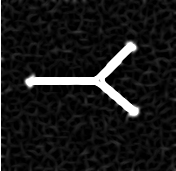
\includegraphics[width=.3\linewidth]{./images/LDE/sim2_ours} \\
		\scriptsize (a) & 		\scriptsize (b) & 		\scriptsize (c)
\end{tabular}
\caption{A simulated image of a Y-junction is shown in (a). The enhancement result using \cite{frangi_vesselness} is shown in (b) and the response at the junction highlighted by the yellow rectangle. (c) The LDE response.  }
\label{fig:demo_junction}
\end{figure}
The dependence on the variables $\theta,\psi_1,\psi_2$ is implied. To incorporate vessels with varying thickness in our solution, a multiscale approach is desirable. Over a range of scales $\mathcal{S}=\{\sigma_{min},\ldots,\sigma_{max}\}$ scale space vesselness response is calculated as follows:
\bea
\mathcal{V}(p)=\max_{\sigma \in \cal S} \mathcal{R}^*(p;\sigma)
\label{eq:vesselness_scalespace}
\eea
The range of scales is problem specific and is determined from prior biological knowledge about the thickness of the vascular structures. 

\begin{figure}[t]
\centering
\renewcommand{\tabcolsep}{0.04cm}
	\begin{tabular}{@{}ccc @{}}
		\includegraphics[width=0.28\linewidth]{./images/LDE/Enhancements/n3_1} &
		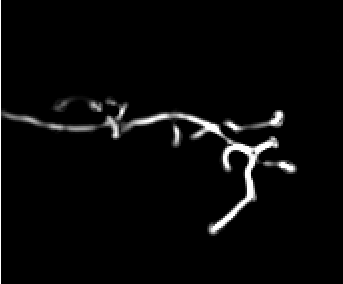
\includegraphics[width=0.28\linewidth]{./images/LDE/Enhancements/n3_1_frangi} &
		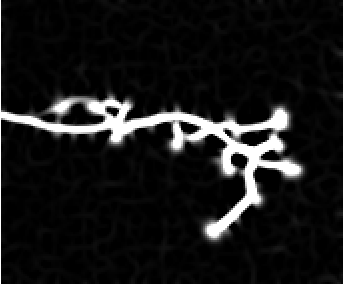
\includegraphics[width=0.28\linewidth]{./images/LDE/Enhancements/n3_1_ours} 
		\\
		\includegraphics[width=0.28\linewidth]{./images/LDE/Enhancements/trial1} &
		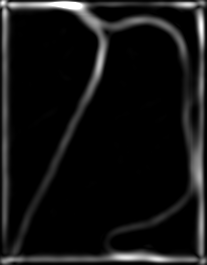
\includegraphics[width=0.28\linewidth]{./images/LDE/Enhancements/trial1_enh_frangi} &
		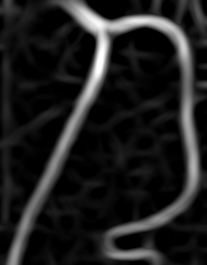
\includegraphics[width=0.28\linewidth]{./images/LDE/Enhancements/trial1_enh_ours} 
		\\
		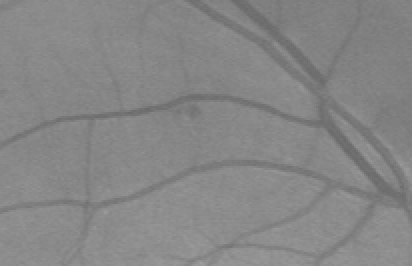
\includegraphics[width=0.28\linewidth]{./images/LDE/Enhancements/vessel_crop_1} &
		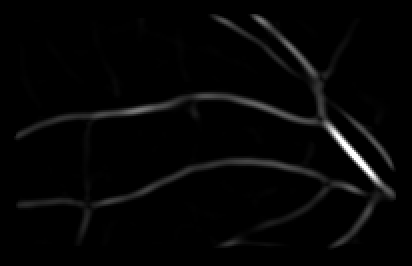
\includegraphics[width=0.28\linewidth]{./images/LDE/Enhancements/vessel_crop_1_enh_frangi} & 		
		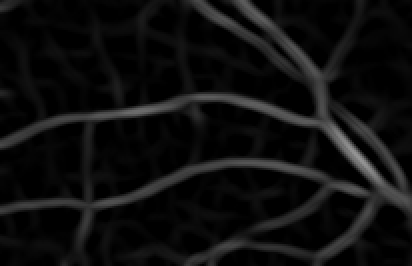
\includegraphics[width=0.28\linewidth]{./images/LDE/Enhancements/vessel_crop_1_enh_ours} 	\\
		\scriptsize (a) & 		\scriptsize (b) & 		\scriptsize (c) 
	\end{tabular}
\caption{(a) Images of filamentous objects. (b) Enhancement results due to Frangi and (c) vessel enhancement using LDE}
\label{fig:enhanced}
\end{figure}

\subsection{Discussion of LDE}
The most significant contribution of this work is in the design of the directional vessel evidence templates. Unlike the standard ridge detector template shown in the first row of Fig.~\ref{fig:templates}, the forward and backward evidence templates in (\ref{eq:r_f}), together with the detector template (\ref{eq:oriented_ridge}), provide an effective way to approximate the vessels as flexible oriented structures, as opposed to the local rigid structure which results from using the detector template only. A set of vessel templates are shown in Fig.~\ref{fig:templates}, second row for illustration. The advantage of using the oriented evidence filters is that complex vessel geometry such as sharp bends and bifurcations can also be handled. While the traditional eigenvalue based method proposed by Frangi\cite{frangi_vesselness} rejects branch points as candidate vessel point (see Fig.~\ref{fig:demo_junction}(b)), LDE is able to tackle the bifurcation by virtue of the local evidence filters (see Fig.~\ref{fig:demo_junction}(c)). 

\section{Edge assisted TuFF}
Adding edge based information to the TuFF variational formulation is quite trivial. The effect of the edge term is to make the contour adhere to the object boundaries, thereby restricting the curve to leak across the boundary. The variational form of geodesic active contour \cite{caselles_GAC} is one way to introduce the edge based energy. This is stated as follows:
\bea
\mathcal{E}_{edge} = \displaystyle \int_\Omega g(\textbf{x})|\nabla H(\phi)|d\textbf{x} \nn \\
\text{where}\quad g(\textbf{x}) = \dfrac{1}{1+|\nabla f(\textbf{x})|^p}
\label{eq:edge_energy}
\eea
Such edge assistance is particularly useful when the  vessels have considerably thicker widths. For narrow vessels, one needs to be conservative while designing the edge attraction term, since it can cause the curve to collapse on to itself. 
The edge based term replaces the contour regularizer part in (TuFF eq). The scalar variable p is manually adjusted to control the influence of the gradient field.  As mentioned in Chapter \ref{GAC_chapter}, the effect of this term is to minimize the geodesic length of the curve, as opposed to the euclidean length minimizer proposed in the original formulation.

\section{Application: automatic crack detection}

To demonstrate the wide applicability of TuFF, we conclude this appendix with some results on a non biological dataset. The problem that we aim to solve here has relevance in the field of civil engineering and involves automated structural health monitoring of concrete structures such as bridges, pavements etc. 

